\documentclass[11pt,a4paper]{scrartcl}
\usepackage[T1]{fontenc}
\usepackage[utf8]{inputenc}
%\usepackage[ngerman]{babel}
\usepackage[ngerman,english]{babel}
\selectlanguage{english}
\usepackage{microtype}
\usepackage{lmodern}
\usepackage{amsmath}
\usepackage{amsfonts}
\usepackage{amssymb}
\usepackage{enumerate}
\usepackage{graphicx}
\usepackage{listings}
\usepackage{color}
\usepackage{url}
\usepackage{multicol}
\usepackage{wrapfig}
\usepackage{amsmath}
\usepackage{tikz}
\usetikzlibrary{arrows}


\begin{document}

\author{Ralf Vogler}
\title{Program Optimization}
\subtitle{Exercise sheet 7}

\maketitle

\section*{Exercise 1: Partially dead code}
\subsection*{1. Analysis}
Contraints and solution:\\
\begin{minipage}[T]{0.5\textwidth}
\begin{align*}
D_1 &\supseteq \emptyset \\
D_2 &\supseteq D_1 \backslash (Use_{x*y} \cup Def_t) \cup \{t = x*y\} \\
D_3 &\supseteq D_2 \backslash Use_{x<y} \\
D_4 &\supseteq D_3 \backslash (Use_{x+1} \cup Def_x) \\
D_5 &\supseteq D_4 \backslash (Use_1 \cup Use_t) \\
D_6 &\supseteq D_2 \backslash Use_{x<y} \\
D_5 &\supseteq D_6 \backslash (Use_8 \cup Def_t) \cup \{t = 8\}
\end{align*}
\end{minipage}
\begin{minipage}[t]{0.5\textwidth}
\begin{tabular}{|c|c|c|}
\hline
& $\mathcal{D} 1$ & $\mathcal{D} 2$\\
\hline
1 & $\emptyset$ & $\emptyset$ \\
2 & $\emptyset \backslash \emptyset \cup \{t = x*y\}$ & $\{t = x*y\}$ \\
3 & $\{t = x*y\} \backslash \emptyset$ & $\{t = x*y\}$ \\
4 & $\{t = x*y\} \backslash (\emptyset \cup \{t = x*y\})$ & $\emptyset$ \\
6 & $\{t = x*y\} \backslash \emptyset$ & $\{t = x*y\}$ \\
5 & $\emptyset \cap \emptyset$ & $\emptyset$ \\
\hline
\end{tabular}
\end{minipage}
\\ \\
Live variables after T7:\\
\begin{tabular}{|c|c|c|}
\hline
& $\mathcal{L}$\\
\hline
1 & $\{x, y\}$\\
2 & $\{x, y\}$\\
3 & $\{x, y\}$\\
3' & $\{t, x\}$\\
4 & $\{t\}$\\
6 & $\{x, y\}$\\
6' & $\emptyset$\\
5 & $\emptyset$ \\
\hline
\end{tabular}

\subsection*{2. Transformation 7}
Original:\\
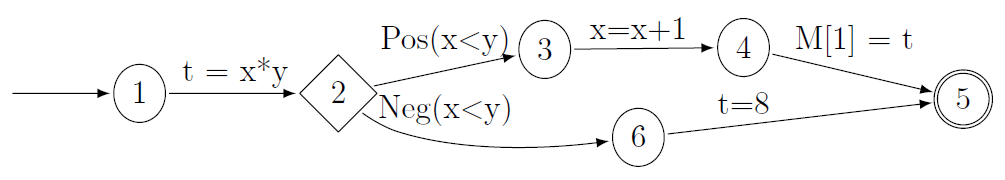
\includegraphics[width=\linewidth]{1org}\\
Transformation T7:\\
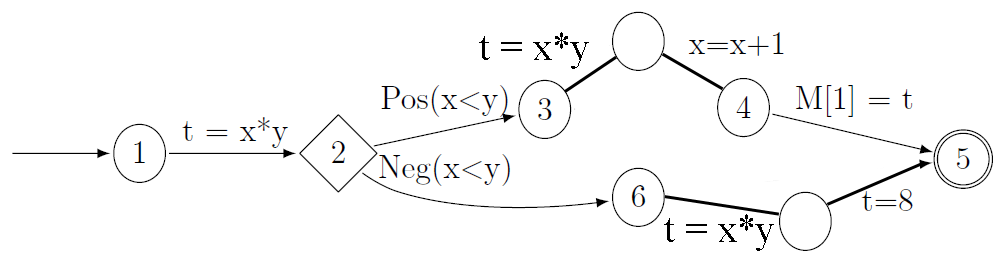
\includegraphics[width=\linewidth]{1}
Transformation T2 (removal of assignments to dead variables):\\
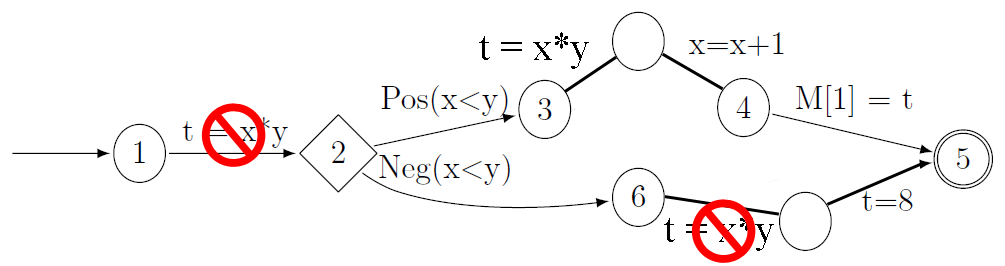
\includegraphics[width=\linewidth]{1_2}
$x = x+1$ could be removed too, because it is dead at point 4.


\section*{Exercise 2: nop-Optimization}
Original:\\
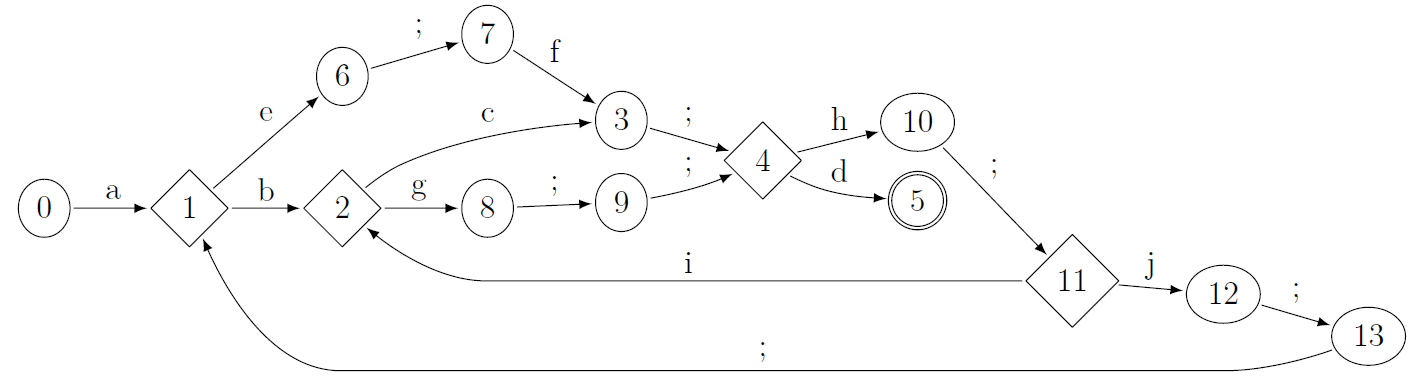
\includegraphics[width=\linewidth]{2org}\\
Transformed:\\
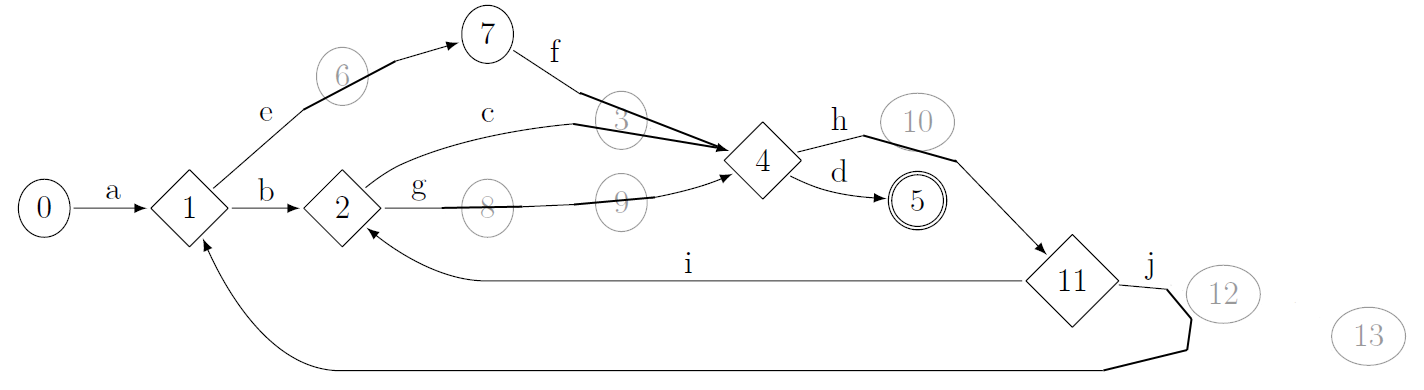
\includegraphics[width=\linewidth]{2}


\section*{Exercise 3: Linearization}
\subsection*{1. Temperatures}
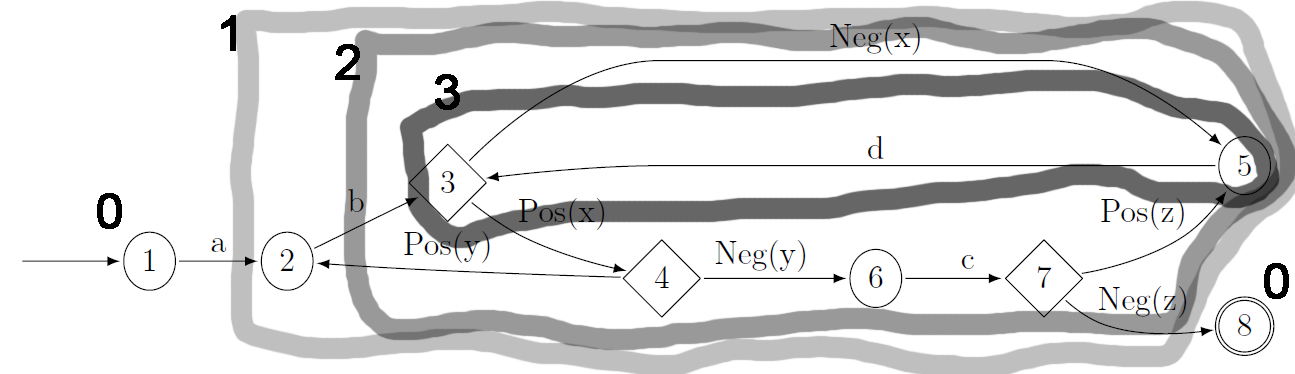
\includegraphics[width=\linewidth]{3}

\subsection*{2. Linearization}
\definecolor{dkgreen}{rgb}{0,0.6,0}
\lstset{
  numbers=left,                   % where to put the line-numbers
  numberstyle=\color{gray},  	  % the style that is used for the line-numbers
  numbersep=5pt,                  % how far the line-numbers are from the code
  keywordstyle=\color{blue},          % keyword style
  commentstyle=\color{dkgreen},       % comment style
}
\begin{lstlisting}[language=C]
a;
b;		// (2)
if(x) goto 6;
d;		// (5)
goto 3;
if(y) goto 2;	// (4)
c;
if(z) goto 4;
halt		// (8)

\end{lstlisting}

\end{document}

















